\documentclass[a4paper,11pt,exos]{nsi} % COMPILE WITH DRAFT


\pagestyle{empty}
\begin{document}

%Exercice 1E11-2



\classe{\premiere spé}
\titre{Ceinture orange 04 - Corrigé}
\maketitle

\begin{exercice}[ : Résoudre une inéquation du second degré]
    Résoudre dans $\R$ les inéquations suivantes :
    \begin{multicols}{2}
        \begin{enumerate}
            \item $-x^2+x+2< 0$
	        \item $4x^2+24x+40\leqslant 0$
        \end{enumerate}
    \end{multicols}
    
\end{exercice}


\begin{enumerate}
    \item Soit $P$ le polynôme défini pour tout $x$ de $\mathbb R$ par $P(x)=-x^2+x+2$.\\On cherche à résoudre $P(x)< 0$.\\Pour cela, on cherche ses racines éventuelles.\\$\Delta = 1^2-4\times(-1)\times2=9$\\$\Delta>0$ donc le polynôme admet deux racines : $x_1 = \dfrac{-b-\sqrt{\Delta}}{2a}$ et $x_2 = \dfrac{-b+\sqrt{\Delta}}{2a}$.\\$x_1 =\dfrac{-1-\sqrt{9}}{-2}=2$\\$x_2 =\dfrac{-1+\sqrt{9}}{-2}=-1$\\On sait qu'un polynôme du second degré est du signe de $a$ à l'extérieur de ses racines.\\Comme $a=-1<0 :$\\On peut résumer le signe du polynôme dans un tableau de signes :\\
        \begin{tikzpicture}[baseline, scale=0.5]
        \tkzTabInit[lgt=10,deltacl=0.8,espcl=5]{ $x$ / 2, signe de $-x^2+x+2$ / 2}{ $-\infty$, $-1$, $2$, $+\infty$}
        \tkzTabLine{  , -, z, +, z, -}
        \end{tikzpicture}
    \\

    Finalement $S=]-\infty;-1[\cup]2;+\infty[$.

    \item Soit $P$ le polynôme défini pour tout $x$ de $\mathbb R$ par $P(x)=4x^2+24x+40$.\\On cherche à résoudre $P(x)\leqslant 0$.\\Pour cela, on cherche ses racines éventuelles.\\$\Delta = 24^2-4\times4\times40=-64$\\$\Delta<0$ donc le polynôme $P$ n'admet pas de racine.\\ Il est toujours du signe de $a=4>0$, donc $P(x)>0$ pour tout $x$ de $\mathbb{R}$.\\ On en déduit $S=\varnothing$.
    \end{enumerate}

\end{document}